\subsection{Example Problems}

\begin{enumerate}

\item You have hopefully learned 4 different search techniques. The
  Bisection Method, the False Position Method, Fixed Point
  Iteration and Newton-Raphson. The function you defined above should
  have a zero somewhere between $-\pi$ to $\pi$. If it doesn't, change your
  frequency $\omega$ so that it does. Then program
  {\bf\underline{ONE}} of the search techniques you've learned and
  have the code solve for the zero. Your function header should look like one of
  the following. 

  \textcolor{blue}{function} xest = mybisection(xL,xR,maxIter) \\
  \textcolor{blue}{function} xest = myfalseposition(xL,xR,maxIter) \\
  \textcolor{blue}{function} xest = myfixedpoint(x0,maxIter) \\
  \textcolor{blue}{function} xest = myNewton(x0,alfa,maxIter) \\

  where xL and xR are your initial guesses for bracketing methods, and
  x0 is your initial guess for the open methods. alfa
  is a parameter you can use to make sure your Newton-Raphson method
  converges properly. maxIter is the
  maximum number of iterations your code will go through. Plot your function
  from problem 1 and the output of your answer on the same graph. The
  code below will plot a square at your solution.  

  plot(xest,0,'ks','MarkerSize',10)

\item You are designing a spherical tank to hold water for a small
  village in a developing country. The volume of liquid it can hold
  can be computed as 

\begin{equation}
V = \pi h^2 \frac{3R-h}{3}
\end{equation}

where V = volume $(m^3)$, h = depth of water (m), and R = the tank
radius (m). If R = 3 m, to what depth must the tank be filled so that
it holds 30 $m^3$? Use three iterations of the false-position to
determine your answer. Employ initial guesses of 0 and R.

\item According to {\it Archimedes Principle}, the buoyancy force is
  equal to the weight of fluid displaced by the submerged portion of
  an object. In order for the sphere to be in a state of equilibrium
  the buoyancy force must be equal and opposite to the force of
  gravity. 

  \begin{equation}
    F_b = \rho_{water}V_{submerged}g = \rho_{sphere}V_{sphere}g
  \end{equation}

  Assume you have a sphere that is submerged into the water. Determine
  the height {\it h} of the portion of the sphere that is above water
  using the bisection method. Use the following values for your
  computation: $R=1~m$,$\rho_{sphere}=200~kg/m^3$,$\rho_{water}=1000
  kg/m^3$. Choose an initial height of 2*R(fully outside the water)
  and a step size of -2*R. Note that the volume of a sphere is simply 

  \begin{equation}
    V_{sphere} = \frac{4}{3}\pi R^3
  \end{equation}

  The volume of the submerged portion is then

  \begin{equation}
    V_{submerged} = \frac{4}{3}\pi R^3 - \frac{\pi h^2}{3}(3R-h)
  \end{equation}

  Perform as many iterations required to reach an error of 1e-2.

\item I would like to know the speed for minimum drag for the aircraft
  that I am currently simulating. Use the Newton-Raphson technique to
  solve for this speed. Assume an initial guess of 30 m/s. The drag of
  an aircraft can be calculated using the following equations.

  \begin{equation}
    \begin{matrix}
      D = \frac{1}2\rho V^2 S(C_{D0} + KC_L^2) \\
      \ \\
      C_L = \frac{2W}{\rho V^2 S} \\
      \end{matrix}
  \end{equation}

  Use the following values in your solution: $\rho = 1.225~kg/m^3$,
  $W=55~N$, $S=0.6558~m^2$, $C_{D0} = 0.028$ and $K=0.0502$. Iterate
  until the change in your velocity values is 1e-2.

\item The mathematical model of a pendulum is set up with a single degree of
freedom. The pendulum can be modeled as a ball of mass ``m", connected
to a rigid massless link of length ``L", as shown in the Figure below. The angle from
the vertical is denoted $\theta$ and can attain values from 0 to
$2\pi$. 
\begin{figure}[htb]
  \begin{center}
    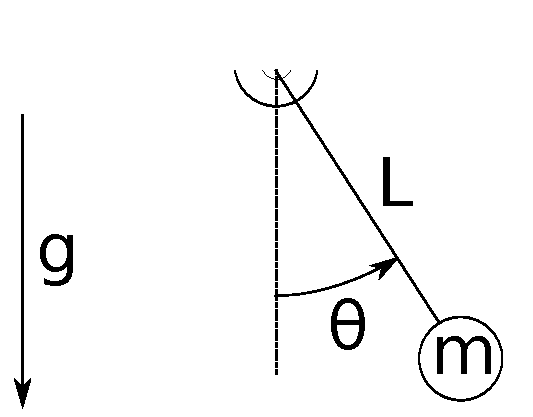
\includegraphics[width=0.4\textwidth]{Graphics/Pendulum.pdf}
  \end{center}
\end{figure}
The equations of motion are second order and are written in terms of
all parameters in the system and are given by the equation below.
\begin{equation}\label{e:full2}
mL^2\ddot{\theta} + mgLsin(\theta) = 0
\end{equation}
It is possible to solve for the analytic solution for small
angles. That is, if $\theta$ is small the approximation
that $sin(\theta) ~= \theta$ is valid. Using this result, the equation above
reduces to the following. Note the equation was also divided by $mL^2$.
\begin{equation}\label{e:simple2}
  \ddot{\theta} + (g/L)\theta = 0
\end{equation}
\noindent The equation above is now simply a spring mass system. The analytical
solution is then
\begin{equation}
\theta(t) = \dot{\theta}_0 \sqrt{\frac{L} g} sin(\sqrt{\frac{g} L}t) + \theta_0 cos(\sqrt{\frac{g} L}t)
\end{equation}

\item Plot the analytical solution for $\theta_0 = \pi/4$ and
$\dot{\theta}_0 = 0$. Assume $m=1~kg$, $g=9.81~m/s^2$, and $L=4~m$.
\ \\

\item Use Euler's integration technique and compute the
numerical solution to the simplified expression in equation
\ref{e:simple2}. Plot the analytical solution on the same graph as the
numerical solution. Did you get the same thing? Is your timestep small enough?
\ \\

\item Use Euler's integration technique and compute the
numerical solution to the full expression in equation
\ref{e:full2}. Plot the analytical solution, the numerical solution
from problem 2 and 3 on the same graph. Do they all look the same? Try
it again for $\theta_0=pi/10$. Do they look the same now? What is happening?
\ \\

\item Bonus: For extra credit create an animation of the pendulum and upload
it along with your word document. Look up movie2avi for help or
request a screen cast. (+50pts)

\item Recall the parachutist falling with an unknown drag
  coefficient. Estimate the drag coefficient using
  the Newton-Raphson technique. Choose an appropriate initial
  guess. Iterate until your percent error is less than 1\% 

\item Perform the same problem as above except this time use the
  bi-section method. Create a plot of your g(K) function to prove that
  your answer is correct. Have the bi-section method iterate until you
  are within 1\%. Make a plot showing the error in your newton-raphson
  estimate, your right bound estimate and your left bound estimate. 
  
\end{enumerate}
